%%%%%%%%%%%%%%%%%%%%%%%%%%%%%%%%%%%%%%%%%
% Beamer Presentation
% LaTeX Template
% Version 2.0 (March 8, 2022)
%
% This template originates from:
% https://www.LaTeXTemplates.com
%
% Author:
% Vel (vel@latextemplates.com)
%
% License:
% CC BY-NC-SA 4.0 (https://creativecommons.org/licenses/by-nc-sa/4.0/)
%
%%%%%%%%%%%%%%%%%%%%%%%%%%%%%%%%%%%%%%%%%

%----------------------------------------------------------------------------------------
%	PACKAGES AND OTHER DOCUMENT CONFIGURATIONS
%----------------------------------------------------------------------------------------

\documentclass[
	11pt, % Set the default font size, options include: 8pt, 9pt, 10pt, 11pt, 12pt, 14pt, 17pt, 20pt
	%t, % Uncomment to vertically align all slide content to the top of the slide, rather than the default centered
	%aspectratio=169, % Uncomment to set the aspect ratio to a 16:9 ratio which matches the aspect ratio of 1080p and 4K screens and projectors
]{beamer}

\graphicspath{{Images/}{./}} % Specifies where to look for included images (trailing slash required)

\usepackage{booktabs} % Allows the use of \toprule, \midrule and \bottomrule for better rules in tables

%----------------------------------------------------------------------------------------
%	SELECT LAYOUT THEME
%----------------------------------------------------------------------------------------

% Beamer comes with a number of default layout themes which change the colors and layouts of slides. Below is a list of all themes available, uncomment each in turn to see what they look like.

%\usetheme{default}
%\usetheme{AnnArbor}
%\usetheme{Antibes}
%\usetheme{Bergen}
%\usetheme{Berkeley}
%\usetheme{Berlin}
\usetheme{Boadilla} %me gusta
%\usetheme{CambridgeUS}
%\usetheme{Copenhagen}
%\usetheme{Darmstadt}
%\usetheme{Dresden}
%\usetheme{Frankfurt}
%\usetheme{Goettingen} %dos dos
%\usetheme{Hannover} %dos dos
%\usetheme{Ilmenau}
%\usetheme{JuanLesPins}
%\usetheme{Luebeck}
%\usetheme{Madrid}
%\usetheme{Malmoe}
%\usetheme{Marburg}
%\usetheme{Montpellier}
%\usetheme{PaloAlto}
%\usetheme{Pittsburgh}
%\usetheme{Rochester} %muy flat
%\usetheme{Singapore}
%\usetheme{Szeged}
%\usetheme{Warsaw}

%----------------------------------------------------------------------------------------
%	SELECT COLOR THEME
%----------------------------------------------------------------------------------------

% Beamer comes with a number of color themes that can be applied to any layout theme to change its colors. Uncomment each of these in turn to see how they change the colors of your selected layout theme.

%\usecolortheme{albatross}
%\usecolortheme{beaver}
%\usecolortheme{beetle}
%\usecolortheme{crane}
%\usecolortheme{dolphin}
%\usecolortheme{dove}
%\usecolortheme{fly}
%\usecolortheme{lily} %default
%\usecolortheme{monarca}
%\usecolortheme{seagull}
%\usecolortheme{seahorse}
%\usecolortheme{spruce}
%\usecolortheme{whale}
%\usecolortheme{wolverine}

%----------------------------------------------------------------------------------------
%	SELECT FONT THEME & FONTS
%----------------------------------------------------------------------------------------

% Beamer comes with several font themes to easily change the fonts used in various parts of the presentation. Review the comments beside each one to decide if you would like to use it. Note that additional options can be specified for several of these font themes, consult the beamer documentation for more information.

\usefonttheme{default} % Typeset using the default sans serif font
%\usefonttheme{serif} % Typeset using the default serif font (make sure a sans font isn't being set as the default font if you use this option!)
%\usefonttheme{structurebold} % Typeset important structure text (titles, headlines, footlines, sidebar, etc) in bold
%\usefonttheme{structureitalicserif} % Typeset important structure text (titles, headlines, footlines, sidebar, etc) in italic serif
%\usefonttheme{structuresmallcapsserif} % Typeset important structure text (titles, headlines, footlines, sidebar, etc) in small caps serif

%------------------------------------------------

%\usepackage{mathptmx} % Use the Times font for serif text
\usepackage{palatino} % Use the Palatino font for serif text

\usepackage[ruled,vlined]{algorithm2e}
%\usepackage{helvet} % Use the Helvetica font for sans serif text
\usepackage[default]{opensans} % Use the Open Sans font for sans serif text
\usepackage[spanish]{babel}
%\usepackage[default]{FiraSans} % Use the Fira Sans font for sans serif text
%\usepackage[default]{lato} % Use the Lato font for sans serif text

%----------------------------------------------------------------------------------------
%	SELECT INNER THEME
%----------------------------------------------------------------------------------------

% Inner themes change the styling of internal slide elements, for example: bullet points, blocks, bibliography entries, title pages, theorems, etc. Uncomment each theme in turn to see what changes it makes to your presentation.

%\useinnertheme{default}
\useinnertheme{circles}
%\useinnertheme{rectangles}
%\useinnertheme{rounded}
%\useinnertheme{inmargin}

%----------------------------------------------------------------------------------------
%	SELECT OUTER THEME
%----------------------------------------------------------------------------------------

% Outer themes change the overall layout of slides, such as: header and footer lines, sidebars and slide titles. Uncomment each theme in turn to see what changes it makes to your presentation.

%\useoutertheme{default}
%\useoutertheme{infolines}
%\useoutertheme{miniframes}
%\useoutertheme{smoothbars}
%\useoutertheme{sidebar}
%\useoutertheme{split}
%\useoutertheme{shadow}
%\useoutertheme{tree}
%\useoutertheme{smoothtree}

%\setbeamertemplate{footline} % Uncomment this line to remove the footer line in all slides
%\setbeamertemplate{footline}[page number] % Uncomment this line to replace the footer line in all slides with a simple slide count

%\setbeamertemplate{navigation symbols}{} % Uncomment this line to remove the navigation symbols from the bottom of all slides

%----------------------------------------------------------------------------------------
%	PRESENTATION INFORMATION
%----------------------------------------------------------------------------------------

\title[SEMINARIO DE INVESTIGACIÓN I]{¿Cómo se hace un mapa conceptual?} % The short title in the optional parameter appears at the bottom of every slide, the full title in the main parameter is only on the title page

%\subtitle{Optional Subtitle} % Presentation subtitle, remove this command if a subtitle isn't required

\author[Luis Ballado]{Luis Ballado} % Presenter name(s), the optional parameter can contain a shortened version to appear on the bottom of every slide, while the main parameter will appear on the title slide

\institute[CINVESTAV]{CINVESTAV - UNIDAD TAMAULIPAS \\ \smallskip \textit{luis.ballado@cinvestav.mx}} % Your institution, the optional parameter can be used for the institution shorthand and will appear on the bottom of every slide after author names, while the required parameter is used on the title slide and can include your email address or additional information on separate lines

\date[\today]{\today} % Presentation date or conference/meeting name, the optional parameter can contain a shortened version to appear on the bottom of every slide, while the required parameter value is output to the title slide

%----------------------------------------------------------------------------------------

\begin{document}

%----------------------------------------------------------------------------------------
%	TITLE SLIDE
%----------------------------------------------------------------------------------------

\begin{frame}
	\titlepage % Output the title slide, automatically created using the text entered in the PRESENTATION INFORMATION block above
\end{frame}

%----------------------------------------------------------------------------------------
%	TABLE OF CONTENTS SLIDE
%----------------------------------------------------------------------------------------

% The table of contents outputs the sections and subsections that appear in your presentation, specified with the standard \section and \subsection commands. You may either display all sections and subsections on one slide with \tableofcontents, or display each section at a time on subsequent slides with \tableofcontents[pausesections]. The latter is useful if you want to step through each section and mention what you will discuss.

%\begin{frame}
%	\frametitle{Contenido} % Slide title, remove this command for no title
	
%	\tableofcontents % Output the table of contents (all sections on one slide)
	%\tableofcontents[pausesections] % Output the table of contents (break sections up across separate slides)
%\end{frame}

%----------------------------------------------------------------------------------------
%	PRESENTATION BODY SLIDES
%----------------------------------------------------------------------------------------

%\section{Introducción} % Sections are added in order to organize your presentation into discrete blocks, all sections and subsections are automatically output to the table of contents as an overview of the talk but NOT output in the presentation as separate slides

%------------------------------------------------
\section{¿Cómo se hace un mapa conceptual?}
\begin{frame}
  \frametitle{¿Qué es un mapa conceptual?}

  \begin{itemize}
    \item Desarrollados por el Prof. Joseph D. Novak en los 70's influenciado por las teorías del aprendizaje significativo de David Ausubel, un destacado psicólogo de la educación.
    \item Herramienta para organizar y representar conocimiento
    \item Permiten una rápida interpretación del material y su relación con el tema de la presentación, ayudando a refinar el mensaje principal a transmitir a la audiencia.
  \end{itemize}

  \begin{figure}
    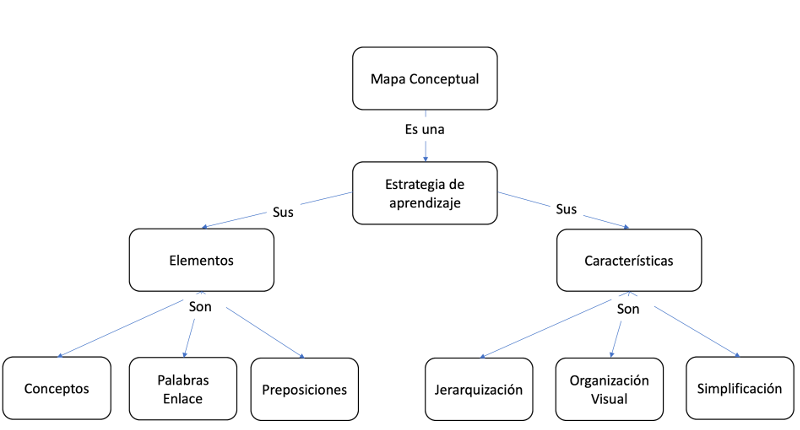
\includegraphics[width=0.7\linewidth]{mapa_conceptual.png}
  \end{figure}
  
\end{frame}

\begin{frame}

  Elementos que debe contener un mapa conceptual
  
  \begin{itemize}
  \item Conceptos
  \item Lineas de unión
  \item Palabras-enlace
  \item Jerarquización
  \item Impacto visual
  \end{itemize}

  \begin{figure}[h]
    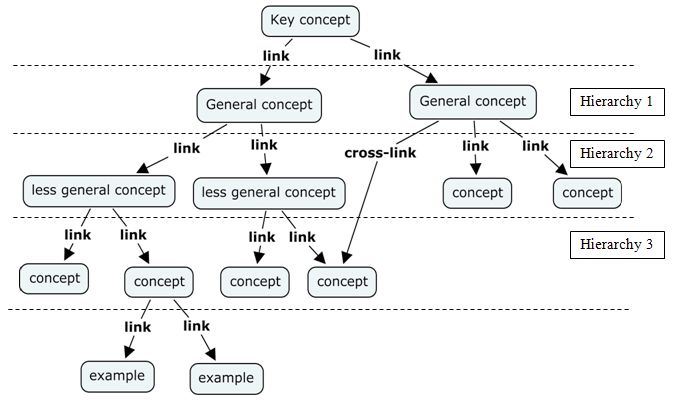
\includegraphics[width=0.7\linewidth]{mapa_c.png}
    \caption{Modelo de Mapa Conceptual Novak $&$ Gowin, 1984}
    \centering
  \end{figure}
  
\end{frame}

\begin{frame}
  \textbf{Conceptos}
  \bigskip % Vertical whitespace

  Un concepto es un término que engloba la generalidad de algo. Es decir, es un término que concretiza toda una idea. Los conceptos de tu mapa conceptual deben ir enmarcados en un recuadro o elipse, de tal manera que se distinga que son los conceptos más esenciales.

  \bigskip % Vertical whitespace
  \textbf{Lineas de unión}\\
  \bigskip % Vertical whitespace
  Indican la relación que existe entre dos o más conceptos. Las lineas pueden ser lineas simples o flechas. Indican una relación bilateral, donde hay un sentido reciproco, mientras que las flechas indican que un concepto se deriva de otro concepto. El concepto principal es el origen y el concepto derivado es el final de la flecha.
  
\end{frame}

\begin{frame}
  \textbf{Palabras enlace}
  \bigskip % Vertical whitespace

  Son las palabras que sirven para unir los conceptos y señalar el tipo de relación existente entre ambos. Las palabras de enlace se escriben en minúsculas fuera de los recuadros, junto a las líneas de unión.

  \bigskip % Vertical whitespace
  \textbf{Jerarquización}\\
  \bigskip % Vertical whitespace
  En los mapas conceptuales los conceptos están dispuestos por orden de importancia. Los conceptos más relevantes ocupan los lugares superiores de la estructura gráfica o bien, se encuentran colocados de tal manera que se note su importancia (letras más grandes, colores más resaltados, etc). Los ejemplos se sitúan en el último lugar y no se enmarcan y tampoco las palabras de enlace.
  
\end{frame}

\begin{frame}
  \textbf{Impacto visual}
  \bigskip % Vertical whitespace

  En palabras de Novak: \textbf{Un buen mapa conceptual es conciso y muestra las relaciones entre las ideas principales de un modo simple y vistoso, aprovechando la notable capacidad humana para la representación visual}\\

  \begin{itemize}
  \item No saturar de colores, procurar combinaciones armónicas de colores. No se trata de armar un arcoiris, sino dar presentación y creatividad.
  \item No usar imágenes de \textbf{relleno} ni saturar de éstas. Las imágenes NO sustituyen los conceptos, sino que los complementan, tampoco es recomendable usar imágenes para todos los conceptos pues corres el riesgo de saturar tu mapa.
  \item Cuidar la tipografía, no usar tipografías distintas a las predeterminadas. 
  \end{itemize}
\end{frame}

\begin{frame}
  \frametitle{Pasos para elaborar un mapa}

  En resumen:\\
  \begin{enumerate}
  \item Identifica las ideas principales y conceptos de cada capítulo.
  \item Agrupa las ideas que estén relaciondadas
  \item Ordena las ideas, puede ser de la más abstracta y general a la más concreta y específica.
  \item Representa y sitúa las ideas en el mapa de acuerdo al orden jerárquico. Enmarca los conceptos con cuadros o elipses.
  \item Conectar y relacionar los conceptos empleando enlaces. Si un concepto deriva a otro indica una flecha, si son del mismo nivel jerárquico utiliza lineas sencillas.
  \item Clarifica las uniones de conceptos e ideas agregando palabras o frases de enlace junto a las líneas de unión.
  \item Dar impacto visual a tu mapa cuidando de no saturar de colores o imágenes
  \end{enumerate}

\end{frame}

\begin{frame}
  \begin{figure}[h]
    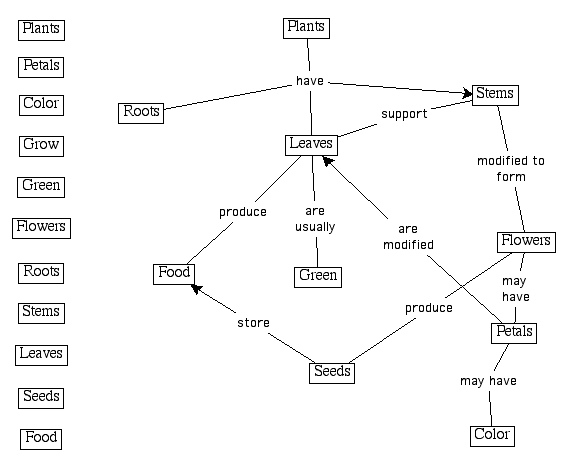
\includegraphics[width=0.7\linewidth]{plants.png}
    \caption{Un buen mapa conceptual}
    \centering
  \end{figure}
\end{frame}

\begin{frame}
  \begin{figure}[h]
    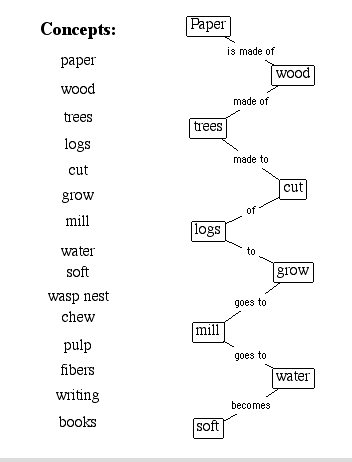
\includegraphics[width=0.5\linewidth]{paper.png}
    \caption{Mapa de frases, no es un buen ejemplo}
    \centering
  \end{figure}
\end{frame}

\begin{frame}
  \begin{figure}[h]
    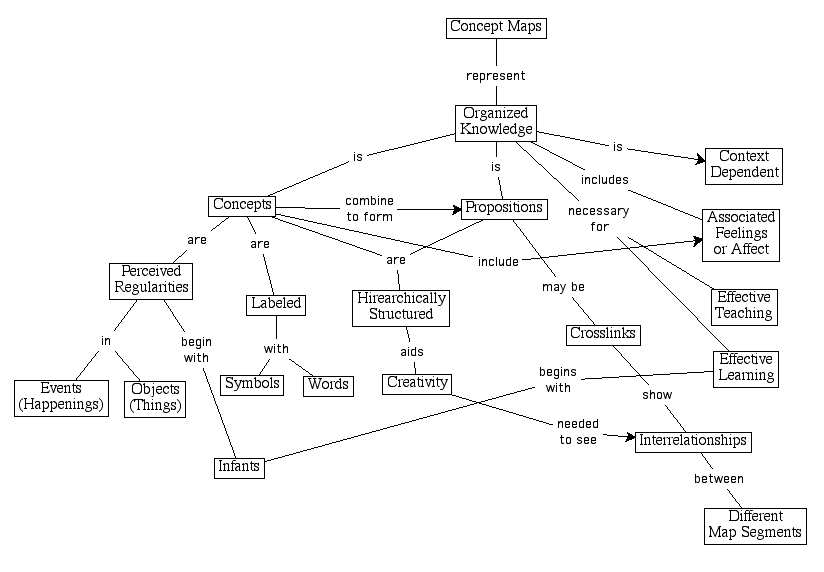
\includegraphics[width=0.9\linewidth]{cmap.png}
    \caption{Un mapa creado por un grupo colaborativo}
    \centering
  \end{figure}
\end{frame}

\begin{frame}{Referencias}
  \begin{thebibliography}{10}
    \setbeamertemplate{bibliography item}[text]
    
    \bibitem{MapaTec}
    Tecnológico de Monterrey, ¿Cómo se elabora un mapa conceptual? \url{http://www.cca.org.mx/ps/profesores/cursos/dahdeca/html/m4/acts_eva/mapa_conceptual.pdf}
  \bibitem{ULondon}
    London Business School, Concept Maps \url{https://teaching.london.edu/development/learning-technologies/concept-maps/}
  \bibitem{Cmap}
    Cmap, The Theory Underlying Concept Maps \url{https://cmap.ihmc.us/docs/theory-of-concept-maps}
  \bibitem{Novak}
    Novak Notes, Concept Maps: What the heck is this? \url{http://cf.psl.msu.edu/ctools/novak.html}
  \end{thebibliography}
\end{frame}
%------------------------------------------------
\end{document} 
